\chapter{Design}
Angelina Scheler \& Christian Pfeiffer

\section{Einleitung}
Aufgabe des Design Teams war das Design der StundenplanApp zu überarbeiten und zu verbessern, unter Berücksichtigung der Apple Design Guideline. Folgende Punkte waren uns dabei wichtig:

\begin{itemize}
\item Neues Design
\item Besseres Design
\item iOS Design
\item Fakultätsfarben
\item Übersichtliches Design
\item Selbsterklärendes Design
\item Onboarding Assistent
\item Widget
\end{itemize}


\section{Stundenplan}
Um das Layout übersichtlicher zu gestalten wurden verschiedene Designkonzepte entworfen.
\subsection{Design Vorschläge}
Die folgenden Abbildungen zeigen die Stundenplan Ansicht in den jeweiligen Fakultätsfarben. Die Stundenplan Informationen wurde in Spalten aufgeteilt. 

\begin{figure}[H]
	\centering
  \frame{ 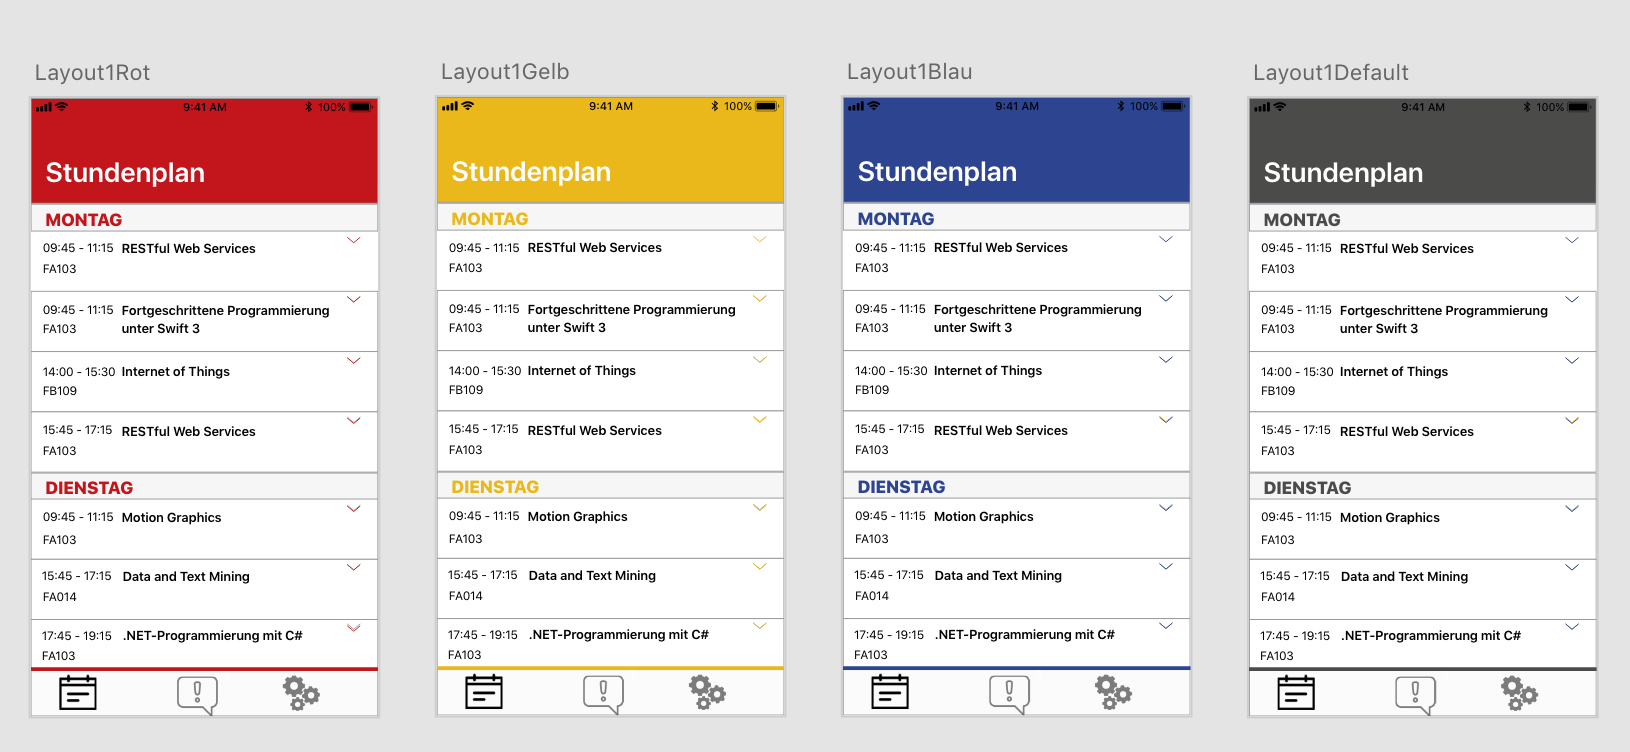
\includegraphics[scale=0.5]{Design1}}
	\caption{Design Konzept 1, Stundenplan Ansicht}
	\label{fig1}
\end{figure}

\begin{figure}[H]
	\centering
  \frame{ 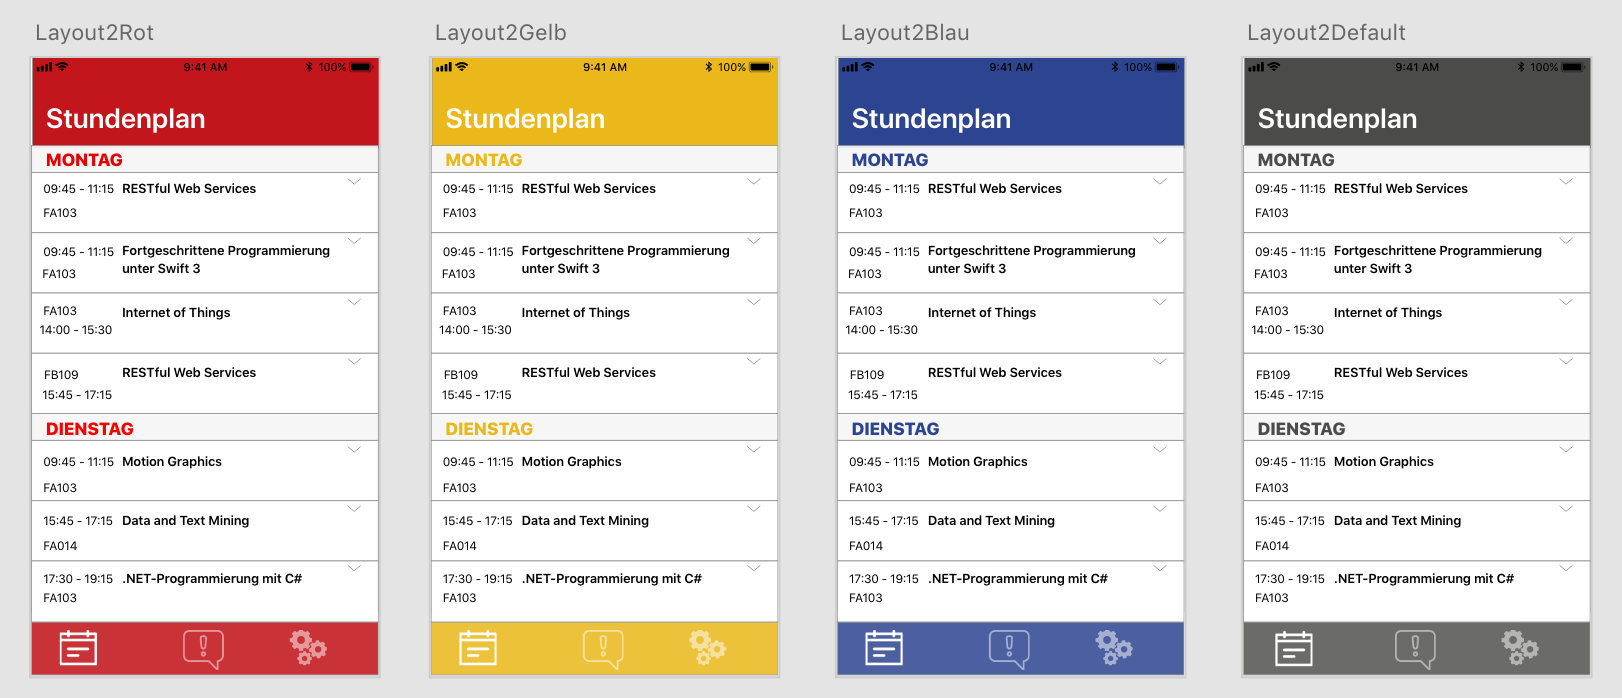
\includegraphics[scale=0.5]{Design2}}
	\caption{Design  Konzept 2, Stundenplan Ansicht}
	\label{fig1}
\end{figure}

\begin{figure}[H]
	\centering
  \frame{ 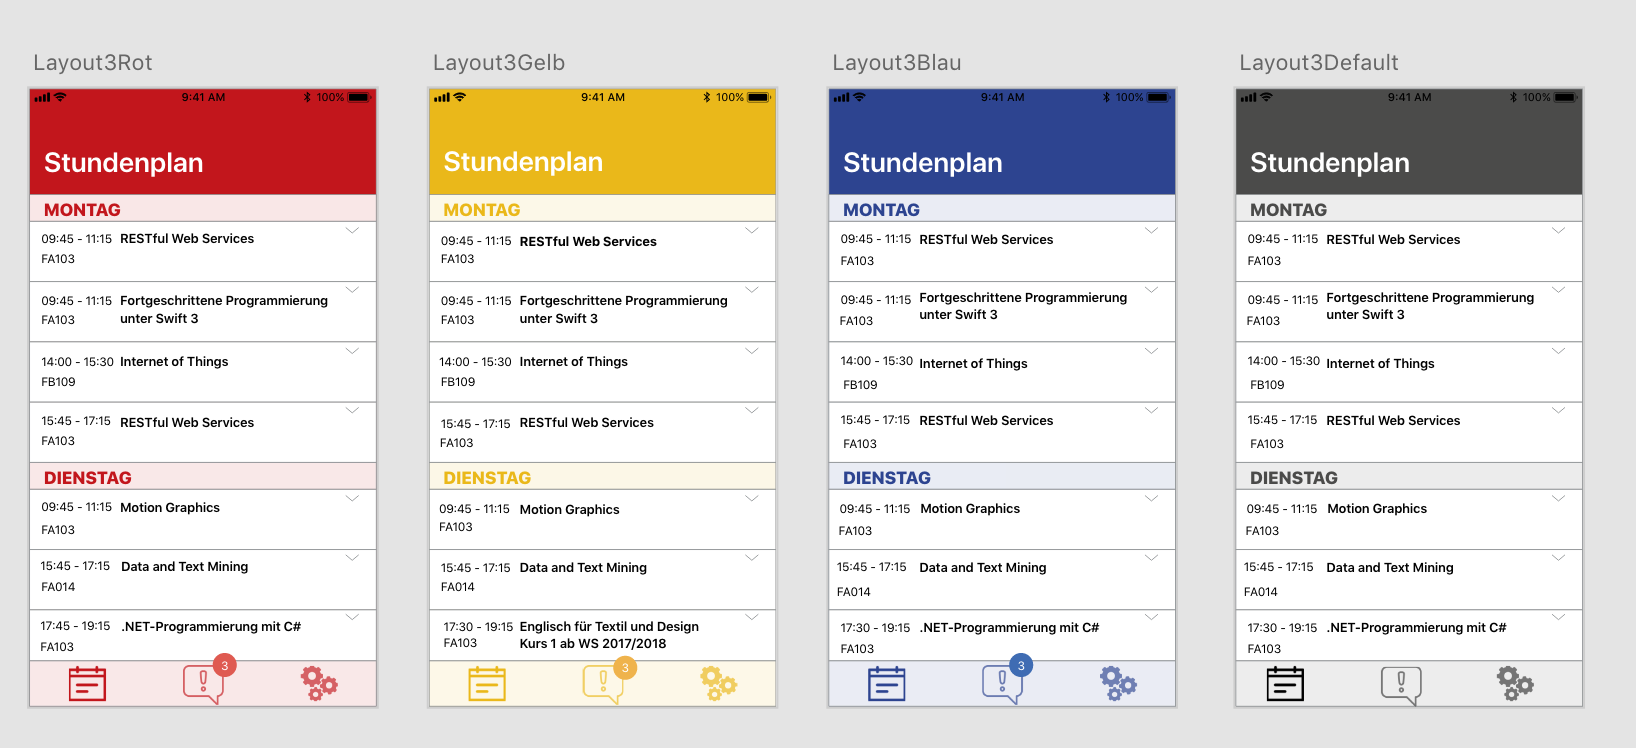
\includegraphics[scale=0.5]{Design3}}
	\caption{Design Konzept 3,  Stundenplan Ansicht}
	\label{fig1}
\end{figure}

\begin{figure}[H]
	\centering
  \frame{ 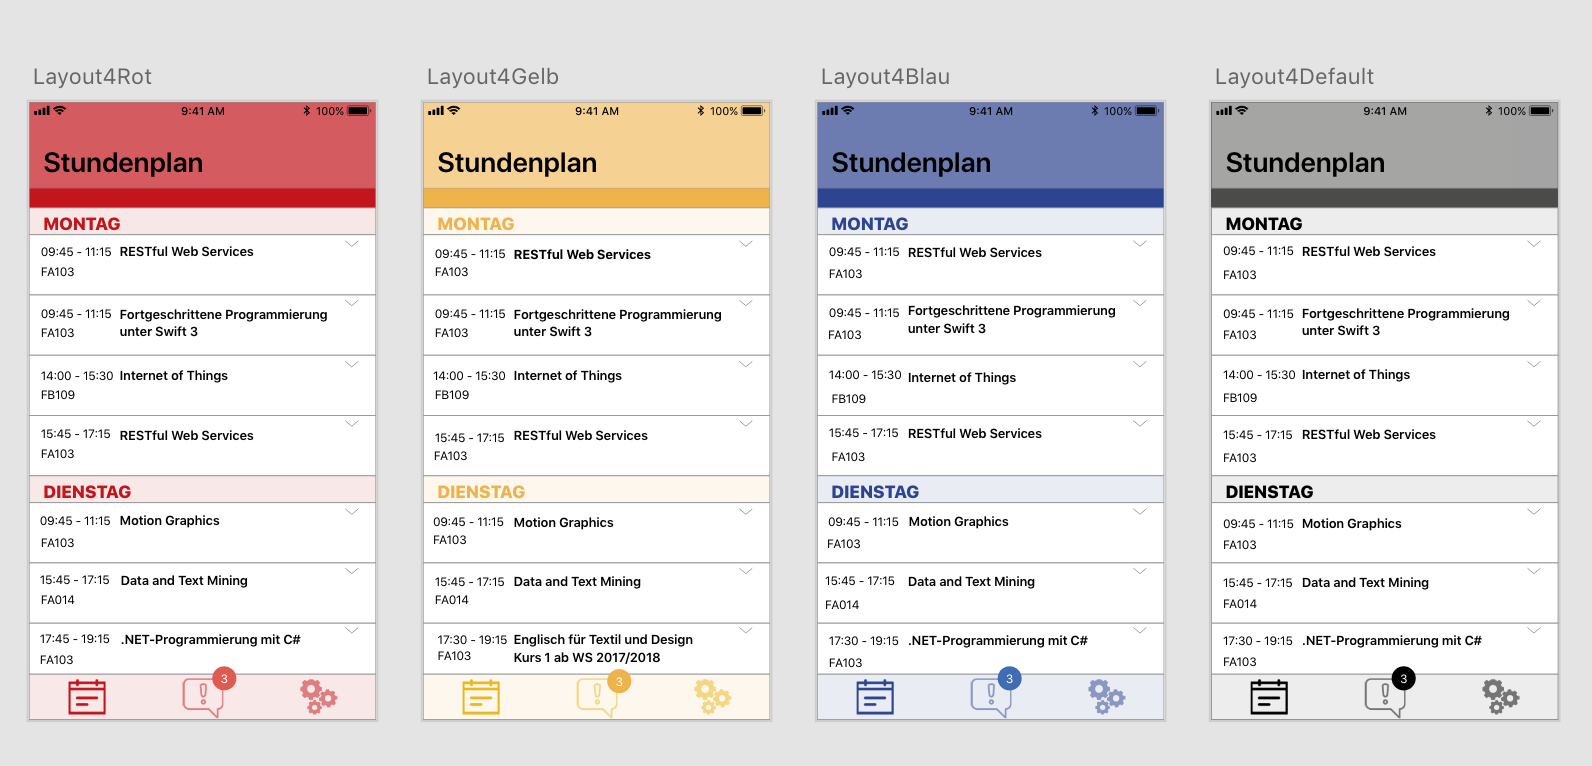
\includegraphics[scale=0.5]{Design4}}
	\caption{Design Konzept 4,  Stundenplan Ansicht}
	\label{fig1}
\end{figure}
\subsection{Finales Design}
Das Finale Design ist ein Kompromiss aus Altem und Neuem Layout, die Fakultätsfarben wurden eingeführt, Informationen übersichtlicher positioniert und farblich angepasst.

\begin{figure}[H]
	\centering
  \frame{ 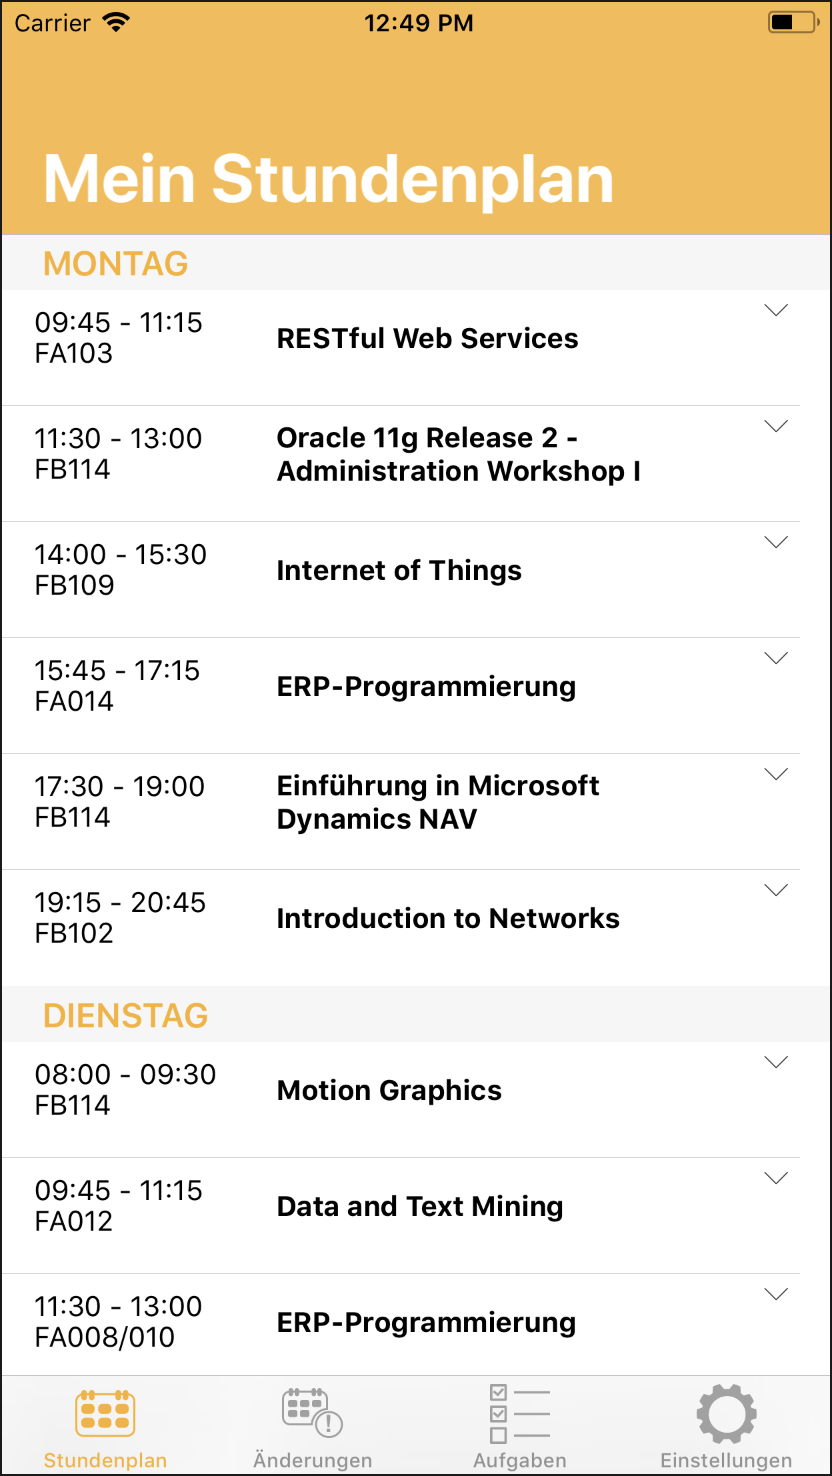
\includegraphics[scale=0.5]{FinalesDesignStundenplan}}
	\caption{Finales Design, Stundenplan Ansicht}
	\label{fig1}
\end{figure}

\begin{figure}[H]
	\centering
  \frame{ 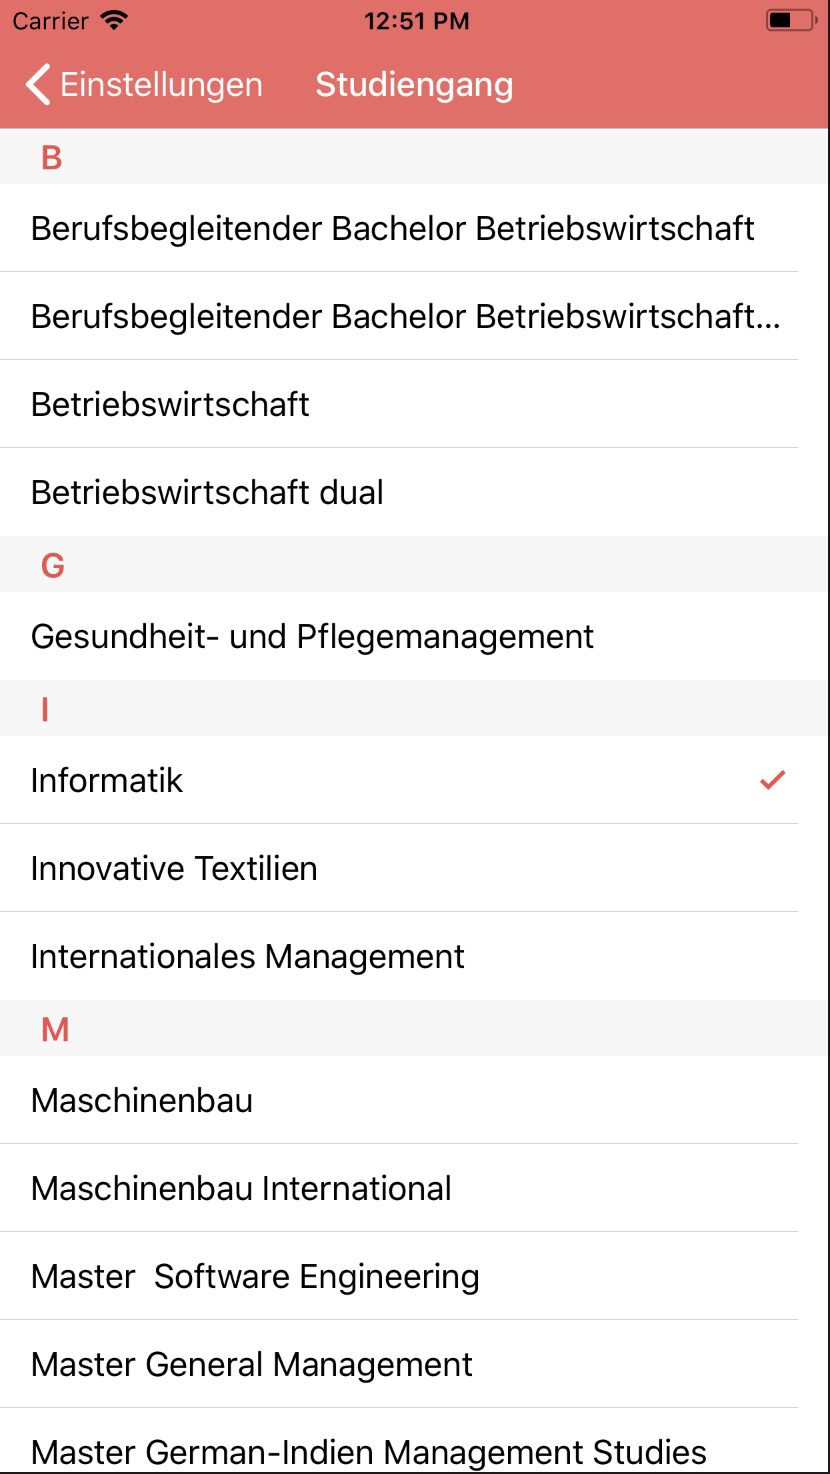
\includegraphics[scale=0.5]{DesignAuswahlStudiengang}}
	\caption{Finales Design, bsp. Auswahl Studiengänge}
	\label{fig1}
\end{figure}




\section{Onboarding}
\section{Einstellungen}
\begin{figure}[H]
	\centering
  \frame{ 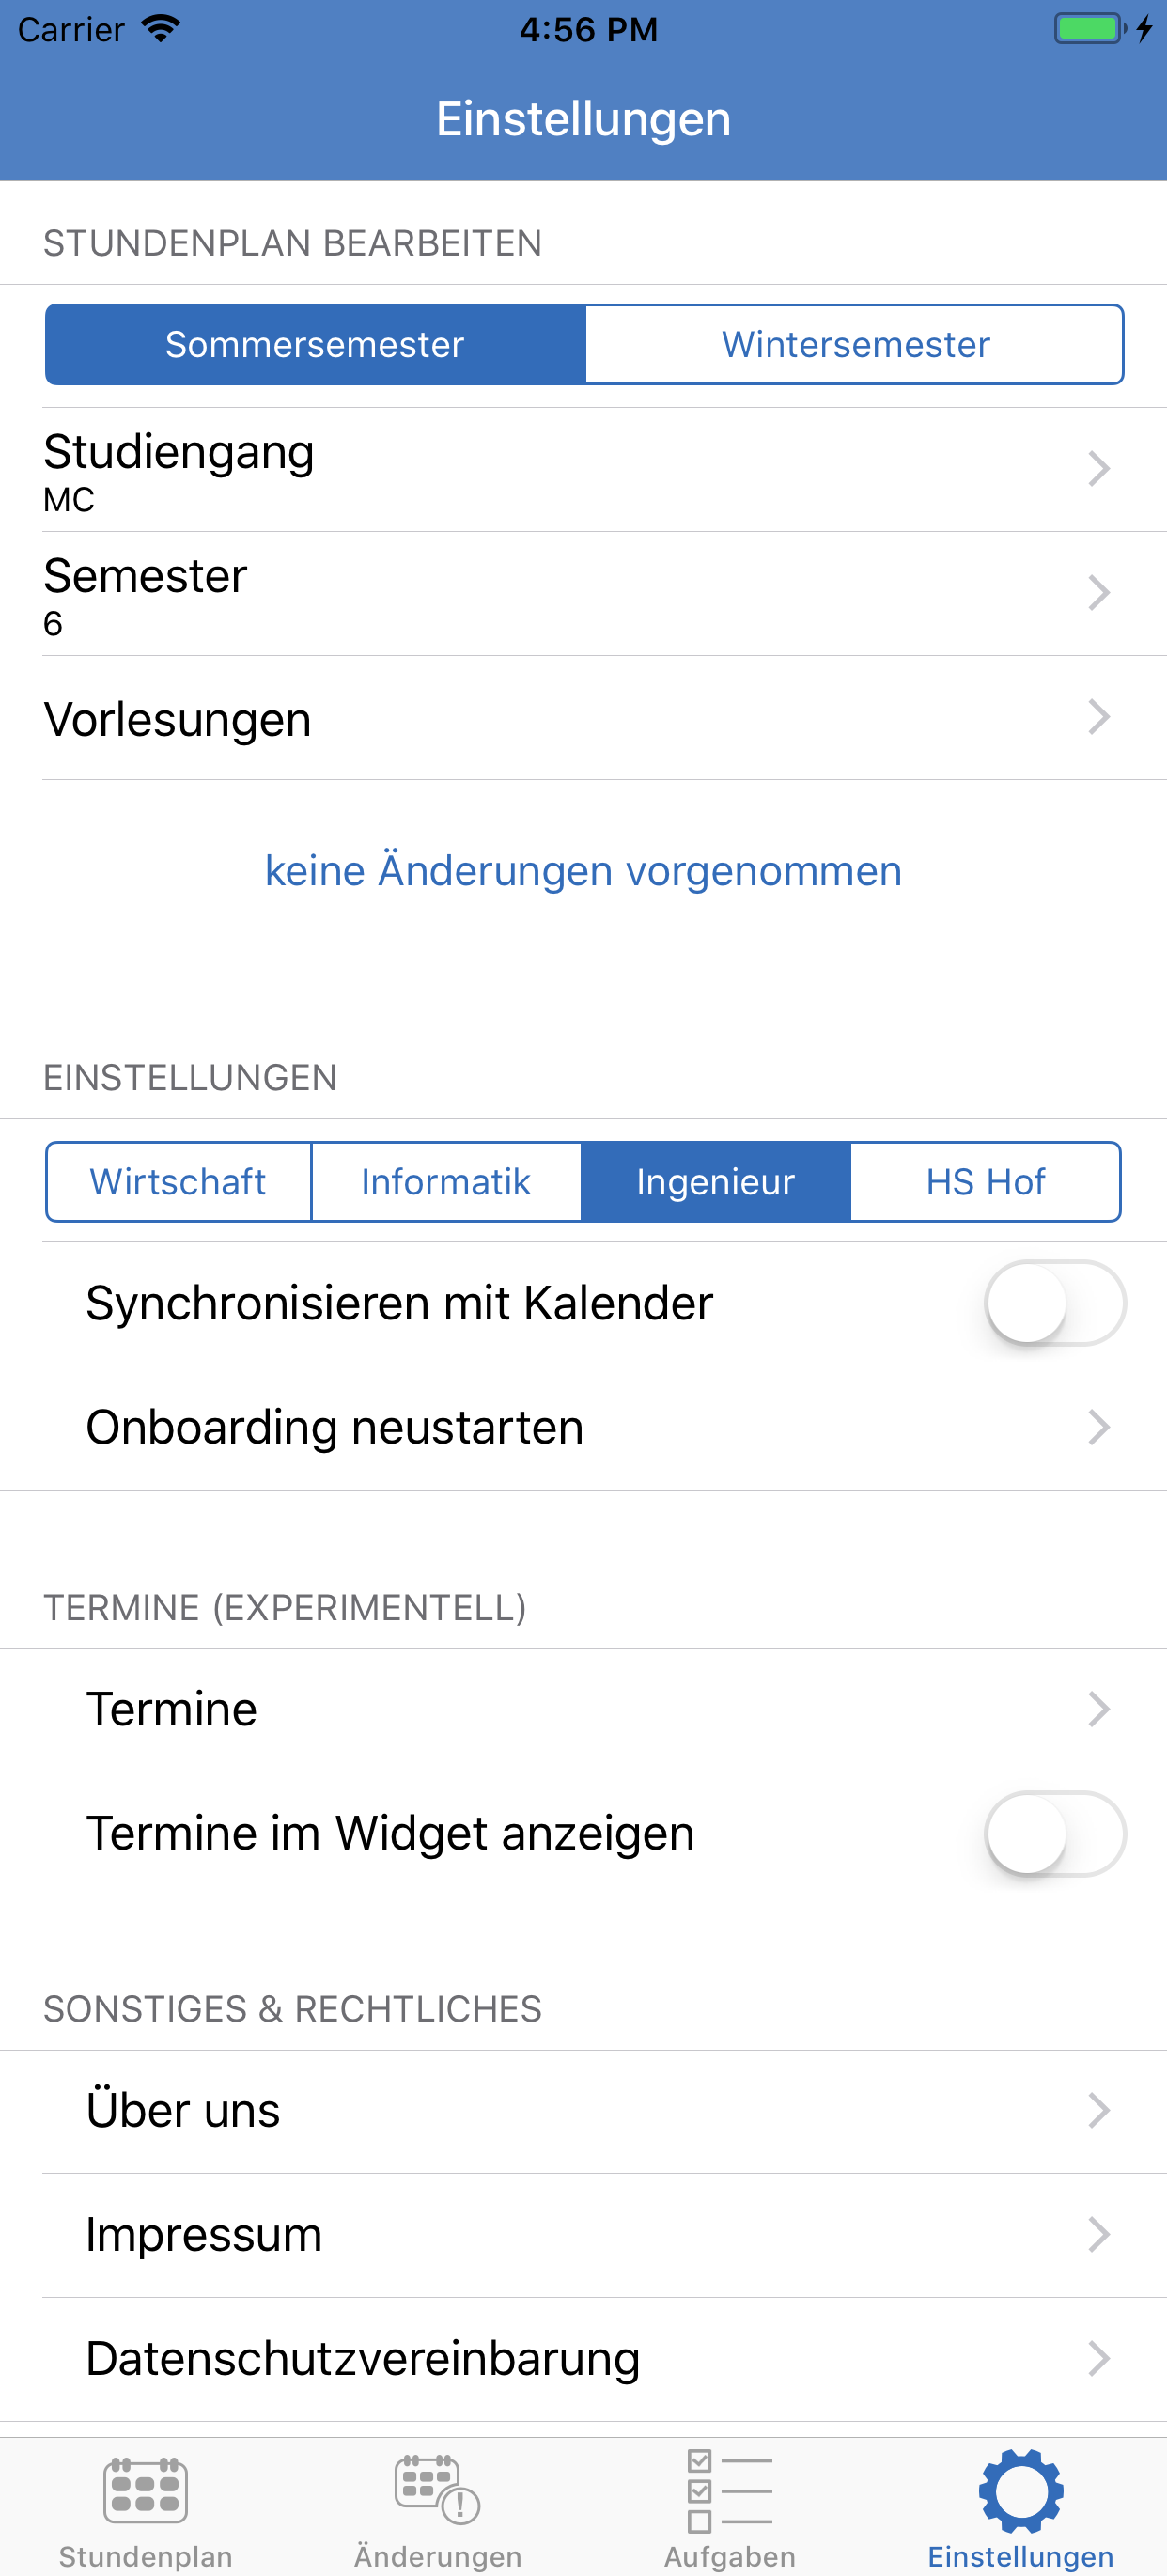
\includegraphics[scale=0.5]{FinalesDesignSettings}}
	\caption{Finales Design, Stundenplan Einstellungen}
	\label{fig1}
\end{figure}

\begin{figure}[H]
	\centering
  \frame{ 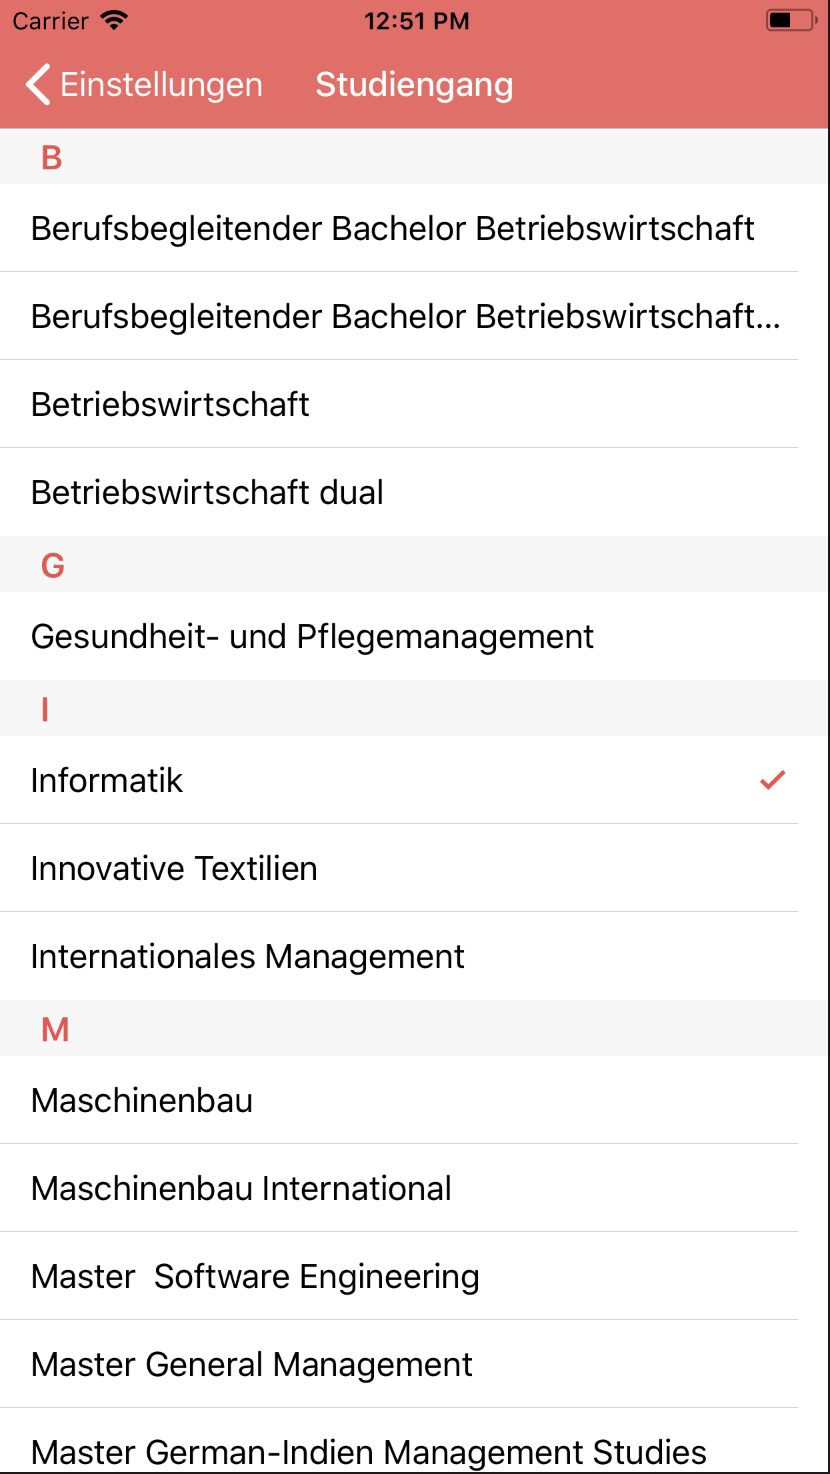
\includegraphics[scale=0.5]{DesignAuswahlStudiengang}}
	\caption{Finales Design, bsp. Auswahl Studiengänge}
	\label{fig1}
\end{figure}

\section{Widget}

\section{demo}
Eine weitere Aufgabe, die unsere Gruppe übernommen hat, war das Onboarding für die Stundenplan App. Im Onboarding kann der Nutzer gleich zum Start der App seine Einstellungen zu Fakultät, Studiengang, Semester, Vorlesung und Kalendersynchronisation vornehmen. Das Onboarding wird gestartet, wenn noch keine Angaben zu den genannten Einstellungen gemacht wurden.

\begin{itemize}
\item Neues Design
\item besseres Design
\item iOS Design
\end{itemize}

\begin{enumerate}
\item Fakultät (die die Farbe der App bestimmt)
\end{enumerate}

\begin{figure}[ht]
	\centering
  \frame{ 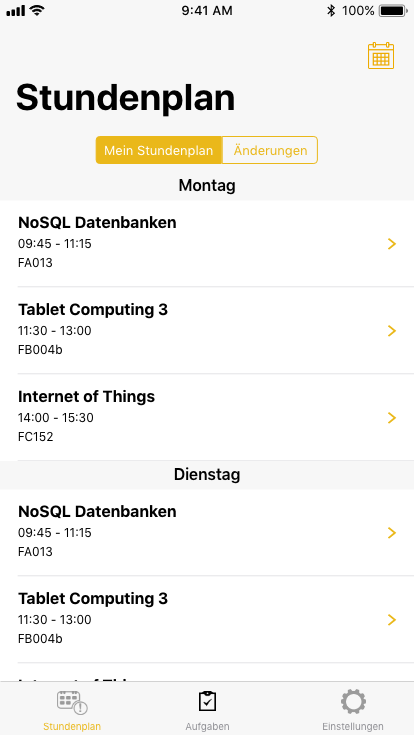
\includegraphics[width=0.4\textwidth]{Mein_Stundenplan} }
	\caption{Mein schönstes Mockup}
	\label{fig2}
\end{figure}

